\section{Mô hình tương tự CLIP: BLIP, ALIGN}
\begin{frame}{6. Các mô hình tương tự CLIP}
\begin{itemize}
    \item ALIGN: \textbf{A} \textbf{L}arge-scale \textbf{I}ma\textbf{G}e and
\textbf{N}oisy-text embedding
    \item BLIP: \textbf{B}ootstrapping \textbf{L}anguage-\textbf{I}mage \textbf{P}re-training for
Unified Vision-Language Understanding and Generation
\end{itemize}
\end{frame}

\begin{frame}{6.1 ALIGN}
\begin{figure}
    \centering
    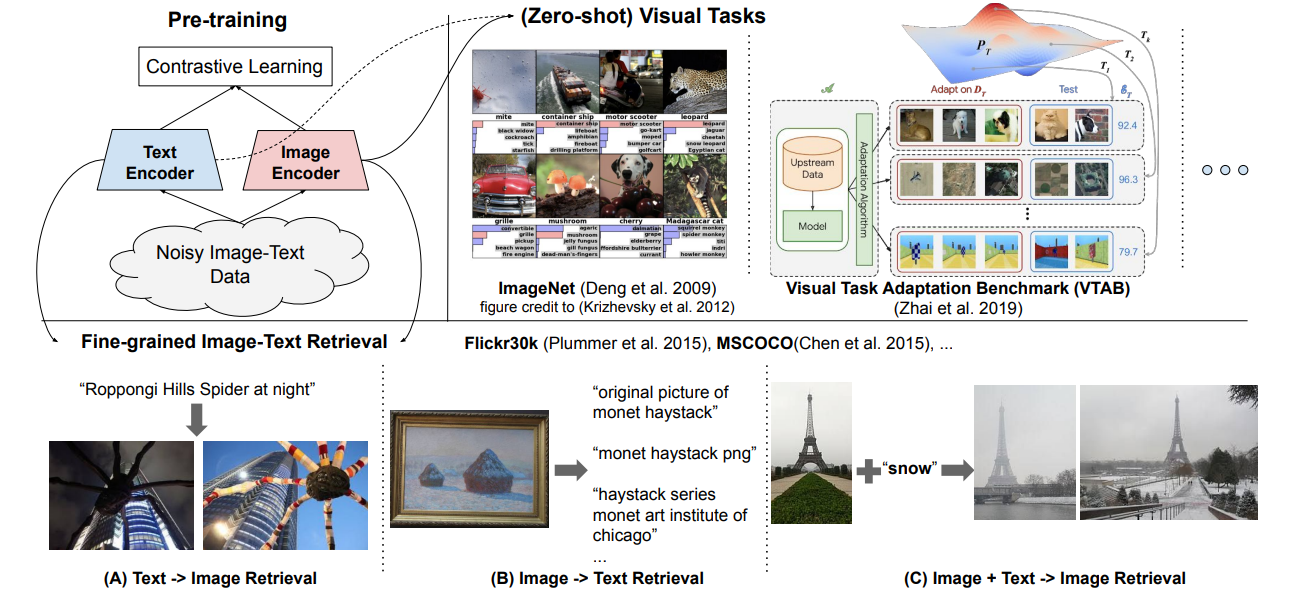
\includegraphics[width=1\linewidth]{img/06-ALIGN.png}
\end{figure}
\end{frame}

\begin{frame}{6.1 ALIGN}
    \begin{itemize}
        \item \textbf{Mục tiêu}: Học biểu diễn vector dùng cho tác vụ thị giác và thị giác-ngôn ngữ với giả thiết: \textbf{Quy mô của dữ liệu có thể bù đắp cho sự nhiễu} của nó.
        \item \textbf{Kĩ thuật:} 
        \begin{itemize}
            \item \textbf{Dữ liệu}: \textbf{1.8 tỷ} cặp ảnh và alt-text thu thập từ web với đặc điểm là rất nhiễu, không hoàn hảo. Sử dụng quy trình lọc đơn giản.
            \item \textbf{Kiến trúc mô hình}: Dual-encoder (EfficientNet và BERT).
            \item \textbf{Loss function}: Contrastive loss InfoNCE.
        \end{itemize}
        \item \textbf{Cách hoạt động:} Huấn luyện đồng thời Image encoder (EfficientNet) và Text encoder (BERT) với mục tiêu kéo gần các vector embedding đúng và đẩy xa các vector embedding sai trong không gian biểu diễn vector chung. 
    \end{itemize}
\end{frame}

\begin{frame}{6.2 BLIP}
\begin{figure}
    \centering
    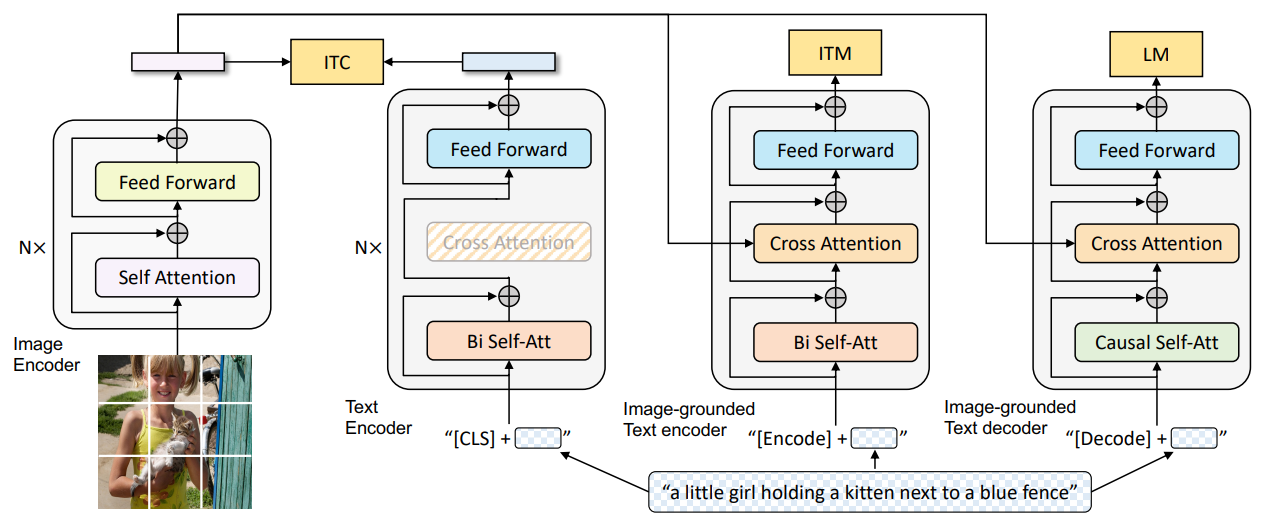
\includegraphics[width=1\linewidth]{img/06-BLIP.png}
\end{figure}
\end{frame}

\begin{frame}{6.2 BLIP}
    \begin{itemize}
        \item \textbf{Mục tiêu}: Làm tốt hai nhiệm vụ \textbf{hiểu} (understanding) và \textbf{sinh} (generation).
        \item \textbf{Kĩ thuật CapFilt:} Tự cải thiện dữ liệu 
        \begin{enumerate}
            \item Huấn luyện BLIP cơ bản, fine-tuning thành 2 model: \textbf{Captioner}, \textbf{Filter}.
            \item Dùng Captioner sinh chú thích cho ảnh, dùng Filter lọc các cặp ảnh-văn bản không khớp.
            \item Kết hợp dữ liệu đã làm sạch, làm giàu này cùng các bộ dữ liệu chất lượng cao để huấn luyện BLIP cuối cùng.
        \end{enumerate}
        \item \textbf{Kĩ thuật Multimodal Mixture of Encoder-Decoder:} 
        \begin{itemize}
            \item Image/Text Encoder: Mã hóa ảnh/văn bản riêng biệt (ITC).
            \item Image-grounded Text Encoder: Kết hợp thông tin hình ảnh vào biểu diễn văn bản (ITM).
            \item Image-grounded Text Decoder: Sinh văn bản dựa trên ảnh đầu vào (LM).
        \end{itemize}
    \end{itemize}
\end{frame}

\begin{frame}{6.3 So sánh CLIP, ALIGN và BLIP}
\begin{table}[H]
{%
\begin{tabular}{|l|p{3.6cm}|p{3.7cm}|p{3.4cm}|}
\hline
\textbf{Tính năng} & \textbf{ALIGN (Google)} & \textbf{CLIP (OpenAI)} & \textbf{BLIP (Salesforce)} \\ \hline
Triết lý & Quy mô dữ liệu bù đắp sự nhiễu & Đặt nền móng cho các tác vụ zero-shot. & Linh hoạt, hiểu sâu ảnh-văn bản. \\ \hline
Kiến trúc & EfficientNet - BERT. & Resnet/ViT-Transformer & MED \\ \hline
Dữ liệu & 1.8 tỷ cặp ảnh-văn bản thô từ web. & 400 triệu cặp ảnh-văn bản (WIT). & Tự tạo và lọc dữ liệu (CapFilt). \\ \hline
Thế mạnh & - NLP đa dạng. \newline - Truy vấn rộng& - Phân loại Zero-shot. \newline - Retrieval image. & - Image captioning. \newline - VQA. \\ \hline
Ứng dụng & Hệ thống tìm kiếm hình ảnh bằng ngôn ngữ tự nhiên, phức tạp. & Tác vụ phân loại nhanh mà không cần fine-tuning. & Ứng dụng đòi hỏi sự hiểu biết chi tiết hình ảnh-văn bản. \\ \hline
\end{tabular}%
}
\end{table}
\end{frame}
